
\section{Ziel}
Ziel des Versuches ist die Untersuchung des Transports von Wärmeenergie entgegen des Wärmeflusses.

\section{Theorie}

\subsection{Güteziffer}
Nach dem zweiten Hauptsatz der Thermodynamik fließt Energie ohne äußeren Einfluss immer vom wärmeren ins kältere
Reservoir, obwohl laut Energiesatz auch der umgekehrte Prozess möglich wäre.
Fügt man dem System jedoch vom außen Energie zu, so kann Energie vom kälteren ins wärmere Reservoir fließen und es gilt
\begin{equation}
  Q_1=Q_2+A ,
\end{equation}
wobei $Q_1$ die zugeführte Energie zum wärmeren Reservoir und $Q_2$ die entnommene Energie aus dem kälteren Reservoir ist.
$A$ ist dabei die Arbeit, die für den Wärmetransport verrichtet werden muss.
Das Verhältnis von $Q_1$ und $A$ wird dabei als Güteziffer $\nu$ bezeichnet.
\begin{equation}
  \nu=\frac{Q_1}{A} \stackrel{\eqref{eqn:QT}}{\Rightarrow} \nu_\text{ideal} = \frac{T_1}{T_1-T_2} \label{eqn:igüte}
\end{equation}
Aus dem zweiten Hauptsatz der Thermodynamik lässt sich ebenfalls der Zusammenhang
\begin{equation}
  \frac{Q_1}{T_1}-\frac{Q_2}{T_2}=0 \label{eqn:QT}
\end{equation}
herleiten.
Dabei wird die Annahme gemacht, dass sich die Temperatur in beiden Reservoiren während der Wärmeübertragung nicht ändert
und der Prozess reversibel abläuft. Die Summe der reduzierten Wärmemengen $\int{\frac{dQ}{R}}$ verschwindet.
Für nicht-reversible Prozesse gilt dagegen:
\begin{equation}
  \frac{Q_1}{T_1}-\frac{Q_2}{T_2} > 0 .
\end{equation}
Aus diesem Zusammenhang folgt, dass die Wärmepumpe besser arbeitet,
wenn die Temperaturdifferenz zwischen den Reservoiren gering ist.
Da \eqref{eqn:QT} zur Berechnung der Güteziffer \nu genutzt wird, muss auch für diese für den realen Fall
umgeschrieben werden:
\begin{equation}
  \nu_\text{real} < \frac{T_1}{T_1-T_2}
\end{equation}
Für eine genauere Bestimmung der Güteziffer muss zunächst der Differenzenquotient $\frac{dT_1}{dt}$ über ein
Zeitintervall $dt$ betrachtet werden.
Für die Wärmemenge $\frac{\symup{d}Q_1}{\symup{d}t}$ ergibt sich:
\begin{equation}
  \frac{\symup{d}Q_1}{\symup{d}t}=\left(m_1 c_\omega + m_k c_k\right)\frac{\symup{d}T_1}{\symup{d}t} .
\end{equation}
Dabei ist $m_1 c_\omega$ die Wärmekapazität des Wassers in Reservoir 1 und $m_k c_k$ die Wärmekapazität der Kupferschlange und
des Eimers.
Für die reale Güteziffer \nu ergibt sich also:
\begin{equation}
  \nu_\text{real}= \frac{1}{N} \frac{\symup{d}Q1}{\symup{d}t},
  \label{eqn:gut}
\end{equation}
Wobei N die momentane Leistung des Kompressors ist.

\subsection{Massendurchsatz}
 Die dem Reservoir 2 entnommende Wärmemenge pro Zeiteinheit lässt sich aus
 \begin{equation}
   \frac{\symup{d}Q_2}{\symup{d}t}=\left(m_2 c_\omega + m_k c_k\right)\frac{\symup{d}T_2}{\symup{d}t}
 \end{equation}
 bestimmen.
 Da die Wärmeübertragung hier durch Verdampfung geschieht, lässt sich der Massendurchsatz durch
 \begin{equation}
   \frac{dQ_2}{dt}=L\frac{\symup{d}m}{\symup{d}t}
   \label{eqn:masse}
 \end{equation}
 bestimmen, wenn die Verdampfungswärme $L$ bekannt ist.

 \subsection{Kompressorleistung}
Für die Arbeit $A_m$, die benötigt wird, um ein Gas eines Volumens $V_a$ auf ein Volumen $V_b$ zu verkleinern, gilt allgemein:
 \begin{equation}
   A_m=\displaystyle\int_{V_b}^{V_a} \rho \symup{d} V
 \end{equation}

Mit der poissonschen Gleichung
\begin{equation}
\rho_a V_a^\kappa=\rho_b V_b^\kappa=\rho V^\kappa
\end{equation}

und
\begin{equation}
  N_\text{mech}=\frac{dA_m}{dt}
\end{equation}
folgt für die gemittelte Leistung:

\begin{equation}
    N_\text{mech} = \frac{1}{\kappa - 1} \cdot \left(p_b \cdot \sqrt[\kappa]{\frac{p_a}{p_b}} - p_a \right) \cdot \frac{1}{\rho} \cdot \frac{\symup{d} m}{\symup{d} t}.
    \label{eqn:leist}
\end{equation}
Dabei $\rho$ ist hier die Dichte des Transportsmediums im gasförmigen Zustand und $\kappa$ das Verhältnis der
spezifischen Wärmekapazität mit konstanten Druck $C_P$ und konstanten der spezifischen Wärmekapazität mit konstanten
Volumen $C_V$.

\subsection{Aufbau und Funktionsweise der Wärmepumpe}
Das Transportmedium in der Wärmepumpe ist hier ein reales Gas, das, ähnlich wie Wasserdampf,
in der Lage ist, beim Verdampfen Energie aufzunehmen und bei Kondensation abzugeben.
Diese Energie wird als Phasenwandlungsenergie bezeichnet.
\begin{figure}[H]
  \centering
  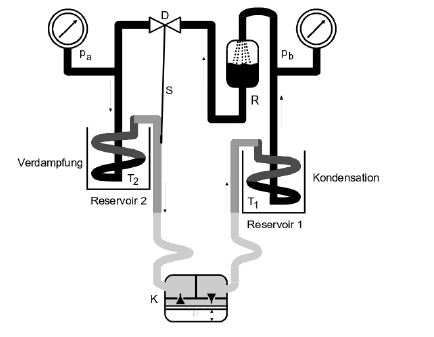
\includegraphics{Text/Bilder/WP.JPG}
  \caption{Aufbau der Wärmepumpe \cite[3]{sample}}
  \label{fig:WP}
\end{figure}
Die Apparatur ist so aufgebaut, dass das Transportmedium unter der Temperatur $T_1$ und dem Druck $p_b$ flüssig ist, während
es unter der Temperatur $T_2$ dem Druck $p_a$ gasförmig ist.
Wird das Drosselventil $D$ geöffnet, verdampft das Transportmedium nach dessen Durchquerung und entzieht dem Reservoir 2
die Verdampfungswärme $L$ pro Gramm Substanz.
Somit ist Reservoir 2 das wärmespendende Reservoir.
Daraufhin wird das Transportmedium im Kompressor $K$ adiabatisch komprimiert.
Dies hat zur Folge, dass die Temperatur des Transportmediums steigt und dieses sich unter dem Druck $p_b$ wieder verflüssigt.
\\
Weitere relevante Bauteile sind der Reiniger $R$ und die Steuerung $S$.
Diese sind nicht zwingend erforderlich, da die Pumpe theoretisch auch ohne diese funktioniert.
Sie werden jedoch genutzt, um den Ablauf zu optimieren.
Der Reiniger $R$ sorgt dafür, dass Blasen, und somit Gasreste, entfernt werden.
Die Steuerung $S$ stellt sicher, dass keine Flüssigkeit in den Kompressor gelangt.
